\documentclass[
  border=5mm,
  convert={
    command={pdftoppm -png -r 600 -singlefile \jobname.pdf \jobname}
  }
]{standalone}
\usepackage{tikz}
\usetikzlibrary{automata,positioning,arrows}
\tikzset{
  ->,
  every state/.style={thick, fill=gray!10, minimum size=1.2cm},
  initial text=All'avvio,
}
\begin{document}
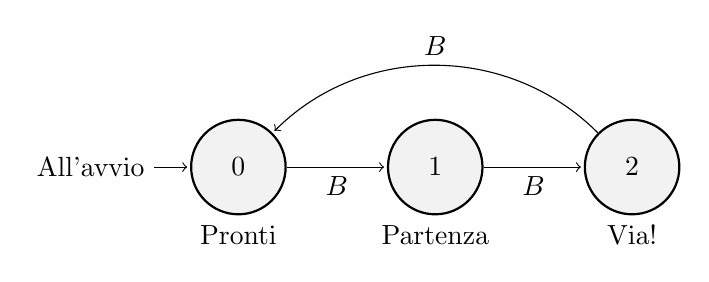
\begin{tikzpicture}[shorten >=1pt, node distance=2.5cm, on grid, auto]
  \node[state, initial, label=below:Pronti] (pronti) {$0$};
  \node[state, right=of pronti, label=below:Partenza] (partenza) {$1$};
  \node[state, right=of partenza, label=below:Via!] (via) {$2$};

  \path[->]
    (pronti) edge[below] node {\(B\)} (partenza)
    (partenza) edge[below] node {\(B\)} (via)
    (via) edge[out=135, in=45] node[above] {\(B\)} (pronti);
\end{tikzpicture}
\end{document}